\documentclass[a4paper,11pt]{article}
% ---- graphiques
\usepackage{ifpdf}
\ifpdf
\usepackage[pdftex]{graphicx}
% for latex2html
\usepackage{html}
\begin{htmlonly}
\newcommand{\includecode}[2]{  \htmladdnormallink{#2}{../../#2} }
\end{htmlonly}
\else
\usepackage{graphicx}
\fi
\usepackage{wrapfig}
\usepackage{color}
%\usepackage{hyperref}



% for accents
\usepackage[latin1]{inputenc}
\usepackage[T1]{fontenc}

\usepackage{algorithm}
\usepackage{algorithmic}

\definecolor{darkgreen}{rgb}{0,0.4,0}
\definecolor{darkblue}{rgb}{0,0,0.4}
\definecolor{darkgray}{rgb}{0.2,0.2,0.2}

% ---- inclusion de codes
\usepackage{listings}
\lstset{showstringspaces=false,tabsize=4,basicstyle=\scriptsize\sffamily,breaklines=true,breakatwhitespace=true,framexleftmargin=5mm, frame=shadowbox, framesep=1pt,rulesepcolor=\color{darkgray},rulesep=.5pt,keywordstyle=\bf\color{blue},commentstyle=\color{magenta},stringstyle=\color{red},numbers=left,numberstyle=\tiny,numbersep=5pt,columns=flexible}

\lstdefinestyle{bash}{language=bash}
\lstdefinestyle{Perl}{language=Perl}
\lstdefinestyle{C++}{language=C++,emph={__global__,__shared__,__syncthreads,blockIdx,threadIdx,float3,float4},emphstyle=\bf\color{darkgreen}}
\lstdefinestyle{DTD}{language=XML}
\lstdefinestyle{XML}{language=XML,usekeywordsintag=false,markfirstintag=true}
%begin{latexonly}
\newcommand{\includecode}[2]{
\lstinputlisting[style=#1]{#2}
}
%end{latexonly}


%\lstnewenvironment{code}{}{}
\lstnewenvironment{code_bash}{\lstset{style=bash}}{}
\lstnewenvironment{code_perl}{\lstset{style=Perl}}{}
\lstnewenvironment{code_cpp}{\lstset{style=C++}}{}
\lstnewenvironment{code_dtd}{\lstset{style=DTD}}{}
\lstnewenvironment{code_xml}{\lstset{style=XML}}{}

\newcommand{\textcode}[1]{{\sf #1}}



%
\newcommand{\sofa}{SOFA}
\newcommand{\todo}[1]{}
\newcommand{\eg}{\textit{e.g.} }

\renewcommand{\vec}[1]{\ensuremath{\mathbf{#1 }}} % vector
\newcommand{\Vx}{\vec{x} } % position vector
\newcommand{\Vv}{\vec{v} } % velocity vector
\newcommand{\Va}{\vec{a} } % acceleration vector
\newcommand{\Vf}{\vec{f}} % force
\newcommand{\Vdv}{\vec{\delta\Vv}} % change of velocity vector (unknown in implicit CG, and used in constraint solver
\renewcommand{\P}{\mat{P} } % projection to a constrained space.

\newcommand{\JNL}{\mathbf{\mathcal{J}} }     % mapping des positions
\newcommand{\J}{\mat J }                 % mapping lineaire
\newcommand{\M}{\mat M }             % matrice de masse
\newcommand{\K}{\mat K }             % matrice de raideur
\newcommand{\B}{\mat B }             % matrice d'amortissement
\newcommand{\G}{\mat G }             % jacobien des contraintes



% ---- inclusion de codes
\definecolor{darkgreen}{rgb}{0,0.4,0}
\definecolor{darkblue}{rgb}{0,0,0.4}
\definecolor{darkgray}{rgb}{0.2,0.2,0.2}


% macros mathematiques
\newcommand{\ma}[1]{\ensuremath{\mathbf {#1}}}
\newcommand{\ve}[1]{\ensuremath{\mathbf {#1}}}

\usepackage{amsmath}
\usepackage{amsfonts}
\usepackage{amssymb}

% character styles
\newcommand{\bm}[1]{\ensuremath{\boldsymbol{{#1}}}}
\newcommand{\mcal}[1]{\mbox{$\mathcal #1$}} % rondes math
\newcommand{\bmcal}[1]{\mbox{\boldmath $\mathcal #1$}} % rondes grasses math
\newcommand{\ensemble}[1]{\mbox{$\mathbb{#1}$}}
\newcommand{\RRR}{\mbox{$\ensemble{R}^3$}} 


% d�finitions
\newcommand{\definition}[2]{\index{#1}{\bf #1}: #2}
\newcommand{\voc}[1]{\index{#1}#1}
\newcommand{\bvoc}[1]{\index{#1}{\bf #1}}

% misc
\newcommand{\EV}[1]{\stackrel{\rightarrow}{#1}}  % espace vectoriel
\newcommand{\EA}[1]{#1}                          % espace affine

% vectors, matrices
%\newcommand{\point}[1]{\mbox{$#1$}}          % un point
\newcommand{\point}[1]{\ensuremath{#1}}          % un point
\newcommand{\mat}[1]{\bm{#1}}         % matrice
\newcommand{\matnm}[3]{\bm{#1_{#2\times #3}}}  % matrice n lignes , m colonnes
\newcommand{\vect}[1]{\bm{#1}}        % vecteur 
%\newcommand{\vecf}[1]{\stackrel{\rightarrow}{#1}}  % vecteur avec fleche
\newcommand{\vecf}[1]{\mbox{$\overrightarrow{#1}$}}  % vecteur avec fleche
\newcommand{\ident}[1]{\bm{I_{#1}}}   % identit� en dimension n
\newcommand{\inv}[1]{#1^{-1}}         % matrice inverse
\newcommand{\psinv}[1]{#1^{+}}        % matrice pseudo-inverse
\newcommand{\transp}[1]{#1^T}         % transpos�e de 1
\newcommand{\trace}[1]{tr(#1)}        % trace
\newcommand{\deter}[1]{\mbox{$|#1|$}}       % determinant
\newcommand{\oppvec}[1]{\mbox{$\left( \vect {#1} \wedge \right)$}}  % operateur matriciel de produit vectoriel

% bases, reperes
\newcommand{\vecin}[2]{\mbox{${}^{#2}#1$}}    % vecteur 1 dans repere 2
\newcommand{\Base}[1]{\ensuremath{\mathcal B_{#1}}} % Symbole du repere 1
\newcommand{\chbase}[3]{\mbox{${}_{#2}^{#3}\mat{#1}$}}  % operateur 1 fait le passage de la base 3 vers la base 2
%\newcommand{\pchbase}[2]{\chbase{\mat{B}}{#1}{#2}}  % matrice de passage de la base 2 vers la base 1
\newcommand{\pchbase}[2]{\chbase{B}{#1}{#2}}  % matrice de passage de la base 2 vers la base 1
\newcommand{\Rep}[1]{\ensuremath{\mathcal R_{#1}}} % Symbole du repere 1
\newcommand{\rep}[1]{\Rep{#1}}                 % Symbole du repere 1
%\newcommand{\pchrep}[2]{\chbase{\mat{F}}{#1}{#2}}  % matrice de passage du repere 1 vers le repere 2, F comme Frame
\newcommand{\pchrep}[2]{\chbase{\bm{C}}{#1}{#2}}  % matrice de passage du repere 2 vers le repere 1

%% Operateur de passage du repere 1 par rapport a 2
%\newcommand{\ChgRep}[2]{\mbox{\boldmath $R_{#1}^{#2}$}}

% rotations	
%\newcommand{\rot}[2]{\mbox{$\mat{R}_{#1,#2}$}}      % rotation vectorielle
\newcommand{\rot}[2]{\ensuremath{\mat{R}_{#1,#2}}}      % rotation vectorielle
\newcommand{\rota}[3]{\mbox{$\mat{R}_{#1,#2,#3}$}}  % rotation affine

% translation
\newcommand{\trans}[2]{\mbox{$\chbase{\vect{t}}{#1}{#2}$}} % passage de #1 vers #2 par une translation, ou translation du repere #2 par rapport au repere #1

% vitesses et acc�l�rations
\newcommand{\VRep}[2]{\mbox{\boldmath $\dot R_{#1}^{#2}$}} % vitesse du repere 1 par rapport a 2 
%\newcommand{\Point}[2]{\mbox{\boldmath ${#1}^{#2}$}}  % Coordonnees d'un point 1 dans un repere 2
\newcommand{\Point}[2]{\mbox{$\vecin{\bm{#1}}{#2}$}}  % Coordonnees d'un point 1 dans un repere 2
\newcommand{\VPoint}[2]{\mbox{\boldmath ${\dot #1}_{/#2}$}} % Vitesse d'un point par rapport � un repere
\newcommand{\APoint}[2]{\mbox{\boldmath ${\ddot #1}_{/#2}$}} % Acceleration d'un point par rapport � un repere

% cinematique du solide
\newcommand{\derivedans}[2]{\mbox{$\dot{#1}^{(#2)}$}}  % derivee du vecteur 1 dans repere 2
\newcommand{\fixedans}[2]{\mbox{$#1_{\in #2}$}}        % vecteur 1 fixe dans repere 2
\newcommand{\vecom}{\mbox{$\bm{\Omega}$}}  % omega de 1 par rapport a 2
\newcommand{\vecrot}[2]{\mbox{$\vecom_{#1/#2}$}}  % omega de 1 par rapport a 2
\newcommand{\accrot}[2]{\mbox{$\dot{\vecom}_{#1/#2}$}}  % omega de 1 par rapport a 2
\newcommand{\vfdans}[3]{\mbox{$\vec V^{#2/#3}_{#1}$}}    % vitesse de 1 fixe dans 2 par rapport a 3
\newcommand{\afdans}[3]{\mbox{$\vec \Gamma^{#2/#3}_{#1}$}}    % acceleration de 1 fixe dans 2 par rapport a 3
\newcommand{\vmdans}[2]{\mbox{$\vec V^{/{#2}}_{#1}$}}    % vitesse de 1 mobile dans 2
\newcommand{\amdans}[2]{\mbox{$\vec \Gamma^{/#2}_{#1}$}}    % acceleration de 1 mobile dans 2

% chaines articulees
\newcommand{\liaison}[2]{\mbox{$\mathcal L_{#1,#2}$}}  % liaison du pere 1 vers fils 2 (et repere intermediaire)
\newcommand{\liaisonprime}[2]{\mbox{$\mathcal L'_{#1,#2}$}}  % deuxieme repere intermediaire de la liaison du pere 1 vers fils 2
\newcommand{\liaisonP}[2]{\mbox{$\mathcal L_{#1,#2}$}}  % Repere dans pere 1 de la liaison vers fils 2 
\newcommand{\liaisonC}[2]{\mbox{$\mathcal L'_{#1,#2}$}}  % Repere dans fils de la liaison du pere 1 vers fils 2 
%\newcommand{\transP}[2]{\pchrep{\liaisonP{#1}{#2}}{#1}}  % Matrice du repere dans pere de la liaison du pere 1 vers fils 2 
%\newcommand{\transC}[2]{\pchrep{\liaisonC{#1}{#2}}{#2}}  % Matrice du repere dans pere de la liaison du pere 1 vers fils 2 
%\newcommand{\transPC}[2]{\pchrep{\liaisonC{#1}{#2}}{\liaisonP{#1}{#2}}}  % matrice de passage entre repere liaison dans fils et repere de liaison dans pere
\newcommand{\transP}[2]{\chbase{C_p}{#2}{#1}}  % Matrice du repere dans pere de la liaison du pere 1 vers fils 2 
\newcommand{\transC}[2]{\chbase{C_c}{#2}{#1}}  % Matrice du repere dans pere de la liaison du pere 1 vers fils 2 
\newcommand{\transPC}[2]{\chbase{C_l}{#2}{#1}}  % matrice de passage entre repere liaison dans fils et repere de liaison dans pere
% \pchrep{fils}{pere} = \liaisonP{pere}{fils}\deplPC{pere}{fils}\liaisonC{pere}{fils}

%topology
\newcommand{\mesh}{{\mathcal M}}
\newcommand{\vertices}{{\mathcal V}}
\newcommand{\edges}{{\mathcal E}}
\newcommand{\triangles}{{\mathcal TR}}
\newcommand{\tetrahedra}{{\mathcal T}}
\newcommand{\controls}{{\mathcal C}}
\newcommand{\nvertices}{{ V}}
\newcommand{\nedges}{{ E}}
\newcommand{\ntriangles}{{ TR}}
\newcommand{\ntetrahedra}{{ TE}}
\newcommand{\ncontrols}{{C}}
\newcommand{\control}{{\mathbf C}}
\newcommand{\degree}{{d}}
\newcommand{\euc}{{\rm I\!R}}
\newcommand{\naturalSet}{{\rm I\!N}}
\newcommand{\sv}{{\mathbf D}}

\newcommand{\pctab  }{\hspace{0.15in}      }  % Pseudo-code indentation.
\newcommand{\code}[1]{ 
\begin{makeimage}
\begin{tabbing} \pctab \= \pctab \= \pctab \= \pctab \= \pctab \= \pctab \= \pctab \kill
#1
\end{tabbing}
\end{makeimage}
}
 % This file is in parent directory. Your TEXI\ncontrolsUTS environment variable must include .. to reach this file. Example: setenv TEXI\ncontrolsUTS ..:../..:${TEXI\ncontrolsUTS}

% ---- format de page A4
	\setlength{\textwidth }{16cm}	% largeur de ligne
	\setlength{\textheight}{23cm}   % hauteur du texte
	\setlength{\oddsidemargin}{0cm} % marge pages impaires
	\setlength{\evensidemargin}{0cm}% marge pages paires
	\setlength{\topmargin}{0cm} 	
	\setlength{\headheight}{14pt} 
	\setlength{\headsep}{0.5cm} 


% Title Page
\title{HOM File Format}
%\author{The \sofa{} team}
\date{June 2017}
\author{Herv\'e Delingette\\ {\small INRIA M\'editerran\'ee, Sophia Antipolis, France}}

\renewcommand{\vertices}{{\mathcal V}}


\newcommand{\Bezier}{{B{\'e}zier }}
\newcommand{\tensorp}{\otimes}
\newcommand{\elem}{{\mathcal T}}

%\newcommand{\degree}{d}

\newcommand{\etal}{{\em et al.}}
\newcommand{\tbiset}{{\mathcal I}}
\newcommand{\tbdiset}{{\mathcal J}}

\newcommand{\tbi}{{\mathbf p}}
\newcommand{\tbip}{{\mathbf p}}
\newcommand{\tbiq}{{\mathbf q}}
\newcommand{\tbimu}{{\bm \mu}}
\newcommand{\elemref}{{\mathcal T}_{\mathrm ref}}
\newcommand{\elemrest}{{\mathcal T}_{\mathbf P}}
\newcommand{\pos}{{\mathbf x}}
\newcommand{\speed}{{\mathbf v}}
\newcommand{\mass}{{\mathbf M}}
\newcommand{\disp}{{\mathbf u}}

\newcommand{\strain}{{\mathbf E}}
\newcommand{\stress}{{\mathbf \sigma}}
\newcommand{\paramt}{\bm  \tau}
\newcommand{\paramti}{\tau}
\newcommand{\param}{ \psi}

\newcommand{\identity}{{\mathbb I}}
%\newcommand{\param}{\bm \psi}

\newcommand{\pointp}{{\mathbf P}}
\newcommand{\tetrap}{{\cal T}_P}







%\newcommand{\euc}{{\rm I\!R}}


\newcommand{\vol}{{\mathcal V}_P}
\newcommand{\stiffness}{{\mathbf K}}
\newcommand{\stiff}{{\mathbf K}}
\newcommand{\force}{{\mathbf f}}

\newcommand{\thicktilde}[1]{\mathbf{\tilde{\text{$#1$}}}}
\graphicspath{./}
\begin{document} 
\maketitle

\section{File Format Description}

\subsection{Constraints on High Order Meshes}

There exists no standard file format to describe high order triangular and tetrahedral meshes of any degree. For instance common file formats such as VTK or GMSH only support triangular and tetrahedral elements of degree 2 (and 3 for GMSH).
The HOM file format aims to fill this need and the SOFA plugin {\em SOFA-HighOrder} provides importer and exporter classes to visualize and use such meshes for scientific computing.

\paragraph{Suitable Element Representations.} In version 1, the HOM file format is only valid for high order simplicial meshes such as high order triangulations and tetrahedralization.  Furthermore, it is only suited for elements where degrees of freedom are represented as control points such as in Bezier or Lagrange elements. Elements like Hermite elements where degrees of freedom are expressed as derivatives are not represented in this format.

\paragraph{Suitable Mesh Representations.} In the HOM format, all elements are of the same type (triangles, tetrahedra) and have the same degree.

\paragraph{Shape functions}. A finite element is the union of its geometric representation (as a collection of control points) and shape functions. In this format, shape functions are not described explicitly but only referenced within a family of generic shape functions such as Bezier or Lagrange.

\subsection{Generic representation of High Order Simplificial Meshes}

In the remainder, we consider high order simplicial meshes of degree $\degree$ consisting of $\nvertices$ vertices, $\nedges$ edges, $\ntriangles$ triangles, $\ntetrahedra$ tetrahedra. The total number of control points is $\ncontrols$ which is defined as :
\begin{equation}
\ncontrols=\nvertices + (\degree-1)\nedges+\frac{(\degree-1)(\degree-2)\ntriangles}{2} +\frac{(\degree-1)(\degree-2)(\degree-3)\ntetrahedra}{6}
\label{eq;np}
\end{equation}


A control point lying on edge can be unambiguously indexed by :
\begin{itemize}
	\item the index $i_e$ in the list of edges of the edge $(v_0,v_1)$ where it is located.
	\item its {\em Edge Index Vector} (EIV) consisting of a pair of integers ${\mathbf p}=(i,j)$ such that $|{\mathbf p}|=i+j=\degree$.
\end{itemize}

Similarly, a control point lying on triangle can be unambiguously indexed by :
\begin{itemize}
	\item the index $i_{tr}$ in the list of triangles of the triangle $(v_0,v_1,v_2)$ where it is located.
	\item its {\em Triangle Index Vector} (TRIV) consisting of a triplet of integers ${\mathbf p}=(i,j,k)$ such that $|{\mathbf p}|=i+j+k=\degree$.
\end{itemize}
Finally, a control point lying on tetrahedron can be unambiguously indexed by :
\begin{itemize}
	\item the index $i_{tet}$ in the list of tetrahedra of the tetrahedron $(v_0,v_1,v_2,v3)$ where it is located.
	\item its {\em Tetrahedron Index Vector} (TETIV) consisting of a quadruplet of integers ${\mathbf p}=(i,j,k,l)$ such that $|{\mathbf p}|=i+j+k+l=\degree$.
\end{itemize}
Finally note that if $d=1$ then $\ncontrols=\nvertices$ and the control points are only the vertices of the simplicial mesh.

\subsection{Format Description}

The HOM file format is a text file that consists of 4 parts :
\begin{enumerate}
	\item {\bf the Header} describing the key parameters of the mesh such the degree of the spline, the dimension of the elements and the nature of the shape functions.
	\item {\bf the control point position} including the number of control points and their coordinates.
	\item {\bf the topology description} including the set of edges, triangles and tetrahedra. 
	\item {\bf the high order control points description} describing the indexing of each control points lying on edges, triangles and tetrahedra. 				
\end{enumerate}

The {\bf header section} consists of 4 lines :
\begin{itemize}
	\item[Line 1] includes the string "HOMF Version 1" and describes the file type and its version.
	\item[Line 2] includes 2 integers "dimEmbedding" and "dimSimplex" where  {\em dimEmbedding} is the dimension of the embedding space and {\em dimSimplex} is the dimension of the simplex element. More precisely, $dimSimplex=2$ for high order triangulations and $dimSimplex=3$ for high order tetrahedral meshes.
	\item[Line 3] includes 1 integer "degree", the degree of the high order element. It has to be greater than 0 $degree\geq 1$, and when $degree=1$ then the mesh is a regular (linear) simplicial mesh.
		\item[Line 4] includes 1 integer "shapeFunctionType" which characterizes the shape function with the following convention:  \begin{center}
\begin{tabular}{|c|c|} \hline 		{\em shapeFunctionType} & Name of shape function \\ \hline 	 0 & Bezier shape function  	 \\ \hline 1 & Lagrange shape function 	 \\ \hline \end{tabular} \end{center}
\end{itemize}


The {\bf control point position part} consists of $\ncontrols+1$ lines : 
\begin{itemize}
\item {\bf Line 1} includes the number of control points $\ncontrols$. 
\item {\bf From Line 1 to Line $\ncontrols+1$} includes $dimEmbedding+1$ float coordinates corresponding to the $dimEmbedding$ coordinates of the control point followed by its weight $w$. For regular (i.e. integral) splines, the weight should be set to $1$. 
\end{itemize}

The {\bf topology description part} consists of the description of the edges, triangles and tetrahedra (if $dimSimplex=3$) of the underlying simplicial mesh. This part consists of  : 
\begin{itemize}
\item {\bf Edge section.} $\nedges+1$ lines where the first line is the number of edges $\nedges$ and the remaining lines describes the two vertices making each edge.
\item {\bf Triangle section.} $\ntriangles+1$ lines where the first line is the number of triangles $\ntriangles$ and the remaining lines describes the three vertices making each triangle.
\item {\bf Tetrahedron section.} $\ntetrahedra+1$ lines where the first line is the number of tetrahedra $\ntetrahedra$ and the remaining lines describes the four vertices making each tetrahedron. This section is only present for high order tetrahedral meshes.
\end{itemize}
The number of lines is therefore $\nedges+\ntriangles+2$ for high order triangulations and $\nedges+\ntriangles+\ntetrahedra+3$ for  high order tetrahedrizations.

The {\bf high order control points description part} aims at describing the indexing of all control points in the high order mesh. Note that $N_{v}$ is not explicitly provided in this format but can be recovered by the knowledge of $\ncontrols$, $\nedges$,$\ntriangles$, $\ntetrahedra$ and $\degree$ from Eq.~\ref{eq;np}.

This {\bf high order control points description part}  consists of :
\begin{itemize}
\item {\bf Edge Control Point section.} It includes $\nedges*(\degree-1)$ lines where each line consists of 4 integers : $i_p, i_e, p_0, p_1$. Index $i_p$ is the index of the control point in the list of control points as provided by the control point position part. Index $i_e$ is the index of the edge in the list of edges as provided in the topology description part. The two indices $(p_0,p_1)$ make the edge index vector (such that $p_0+p_1=\degree$) which positions the control point on the edge.
\item {\bf Triangle Control Point section.} It includes $\ntriangles*(\degree-1)*(\degree-2)/2$ lines where each line consists of 5 integers : $i_p, i_{tr}, p_0, p_1, p_2$. Index $i_p$ is the index of the control point in the list of control points as provided by the control point position part. Index $i_{tr}$ is the index of the triangle in the list of triangles as provided in the topology description part. The three indices $(p_0,p_1,p_2)$ make the triangle index vector (such that $p_0+p_1+p_2=\degree$) which positions the control point on the triangle.
\item {\bf Tetrahedron Control Point section.} It includes $\ntetrahedra*(\degree-1)*(\degree-2)*(\degree-3)/6$ lines where each line consists of 6 integers : $i_p, i_{tet}, p_0, p_1, p_2, p_4$. Index $i_p$ is the index of the control point in the list of control points as provided by the control point position part. Index $i_{tet}$ is the index of the tetrahedron in the list of tetrahedra as provided in the topology description part. The four indices $(p_0,p_1,p_2,p_3)$ make the tetrahedron index vector (such that $p_0+p_1+p_2+p_3=\degree$) which positions the control point on the tetrahedron.
\end{itemize}

\subsection{Example}

In Fif.\ref{fig:HOMFormat} an example of a high order mesh consisting of 2 cubic Bezier triangles is exported in a HOM file format. There are $\ncontrols=16$ control points that are split into $\nvertices=4$ vertices, $\nedges*2=10$ edge control points and $\ntriangles*1=2$ triangle control points.  The edge index vectors are either $(1,2)$ or $(2,1)$ and triangle index vectors are $(1,1,1)$.

\begin{figure}[!htbp]
	\centering
\mbox{    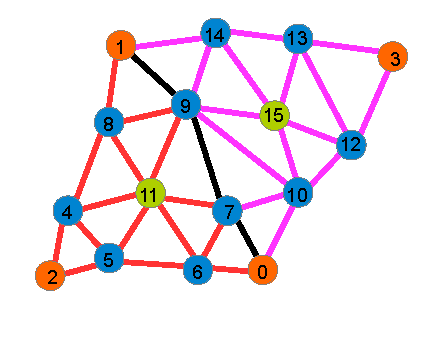
\includegraphics[width=0.40\textwidth]{exampleHOM}}
\mbox{		  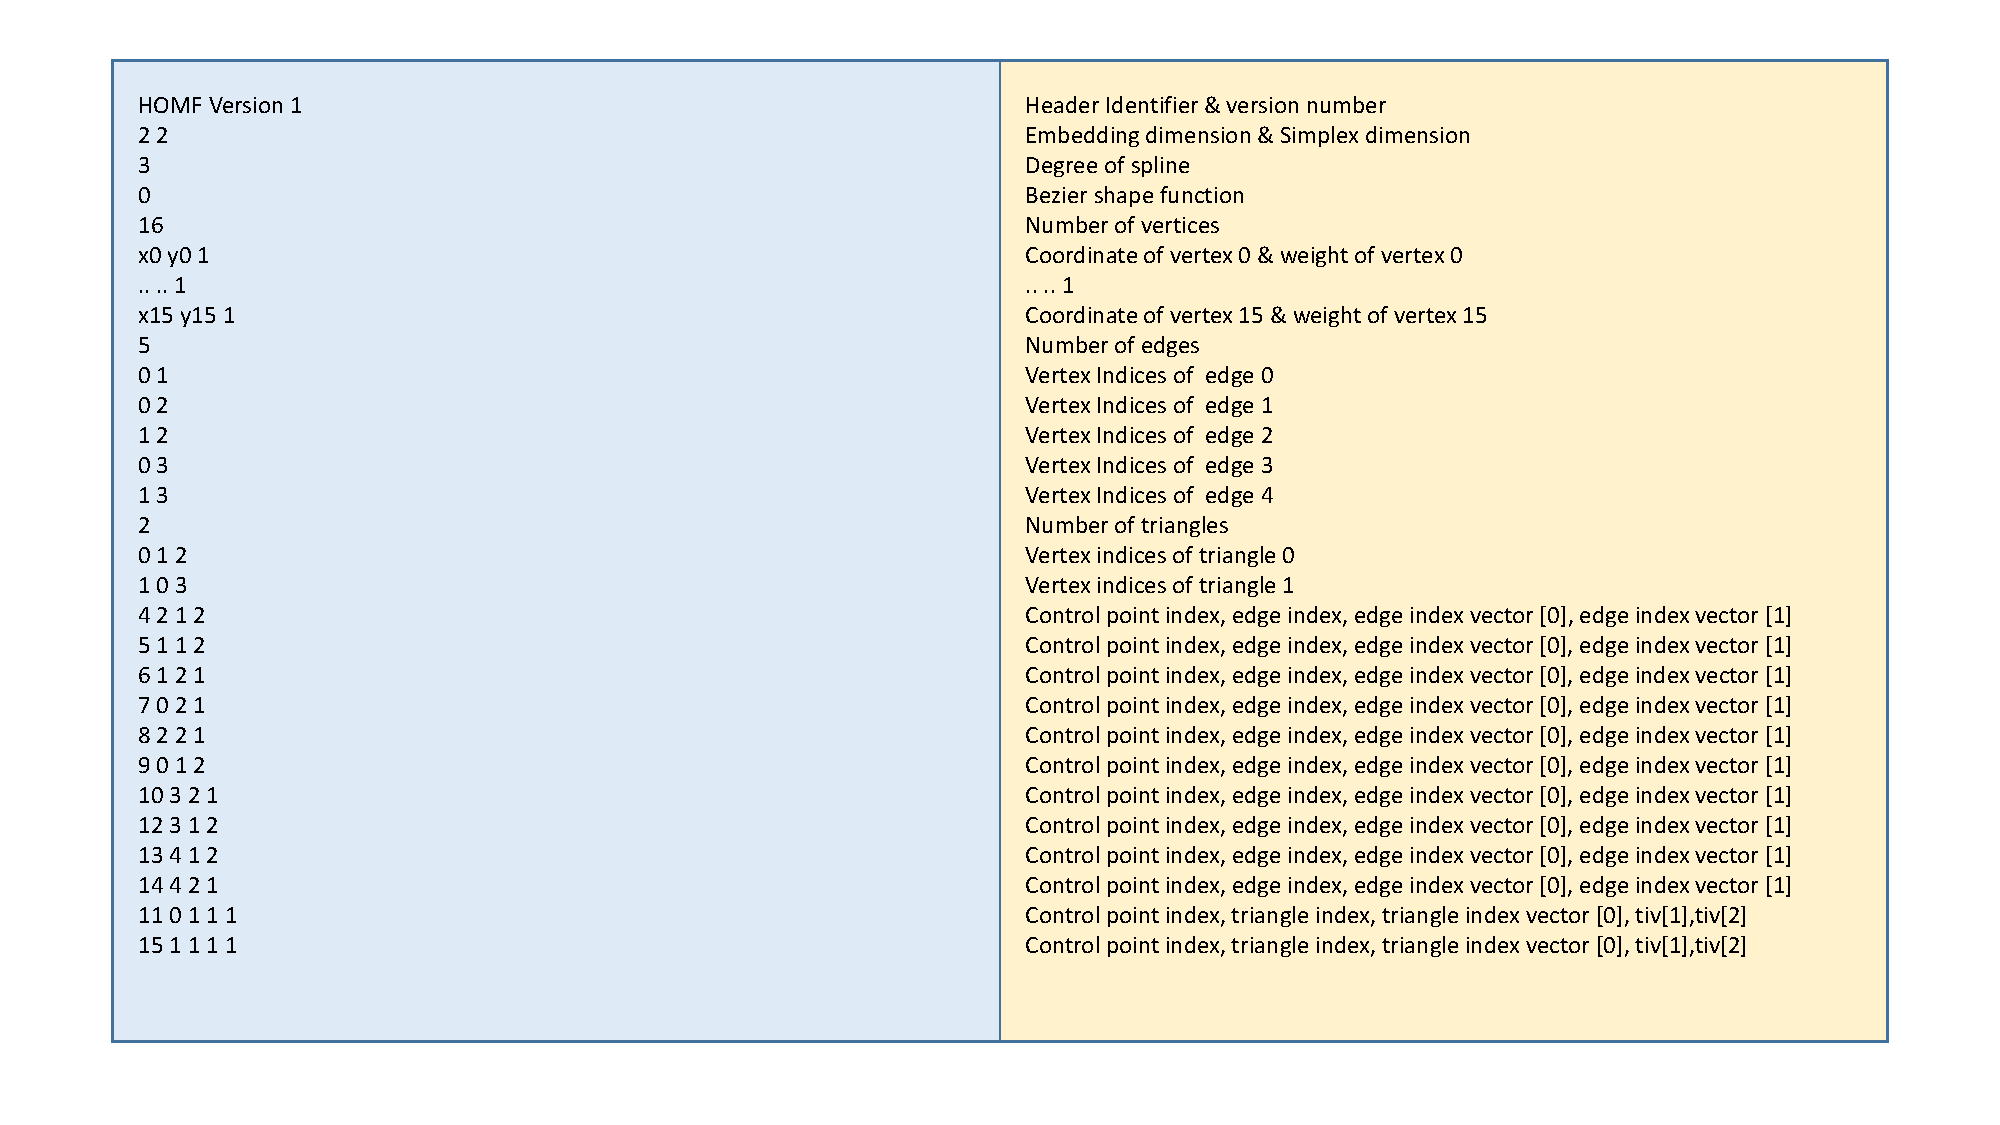
\includegraphics[width=0.80\textwidth]{HOMFormat}}
	\caption{(Top) Example of a high order mesh consisting in two cubic triangles sharing an edge. Orange vertices are vertices of the 2 triangles, blue vertices are edge control points and green vertices are triangle control points. (Bottom) Left panel corresponds to the HOM file while the right panel is the explanation of the corresponding line.}
	\label{fig:HOMFormat}
\end{figure}

\section{SOFA Importer and Exporter Classes}

\subsection{Importer Class : HOMFFileExporter}

To export a high order mesh in HOM format from a SOFA scene, one should use the component HOMFFileExporter. The component can export a mesh at the beginning of the simulation, or at the end, or every n steps. The object HOMFFileExporter should be placed in the same node or below the object  HighOrderTriangleSetTopologyContainer (or HighOrderTetrahedronSetTopologyContainer) associated with the mesh. Furthermore, it has also to be placed in the same node or below the object BezierTriangleSetGeometryAlgorithms ( or BezierTetrahedronSetGeometryAlgorithms) or similar classes for different shape functions.

Important fields of this object are :
 \begin{center}
\begin{tabular}{|c|l|} \hline 		{\em Field} & Description \\ \hline 
	 filename & base file name of exported file  	 \\ \hline 
	overwrite & \tiny  When false as default create a new file at each export, with suffix added to the filename 	 \\ \hline
	exportEveryNumberOfSteps & \tiny  the number of steps between 2 exports, if 0 as default then no export is performed  \\ \hline
	formatVersion & the format version of the HOM file \\ \hline
		exportAtBegin & if the file should be exported before any iteration  \\ \hline
				exportAtBegin & if the file should be exported when the simulation is finished  \\ \hline
	\end{tabular} \end{center}
	
	See examples in GenerateSphere.xml 

\subsection{Exporter Class : MeshHOMFLoader}

To import a high order mesh in HOM format, use component MeshHOMFLoader. As input it only requires the field "filename" which is self explanatory. As output, it fills the fields "position", "position2D", "edges", "triangles", "tetrahedra", "weights", "inputHighOrderEdges", "inputHighOrderTriangles", 
"inputHighOrderEdgePositions", "inputHighOrderTrianglePositions", "inputHighOrderTetrahedronPositions". Those fields can then be connected to the classes HighOrderTetrahedronSetTopologyContainer and HighOrderTriangleSetTopologyContainer to initialize the mesh.

See TestLoaderHOMFFile2D.xml and TestLoaderHOMFFile3D.xml as examples.



\end{document}          

